\chapter{Implementation \label{implementation}}

In this chapter, we present an overview of an interpreter designed for the language presented in chapter~\ref{language}.
The algorithm for checking composition, the implementation of activations, the implementation of heaps, and the scheduler are presented in detail.

\paragraph{Interpreter organization.}
The interpreter has an orthodox design consisting of a scanner, a parser, a sequence of semantic checks, a code generation phase, composition checks, and a execution phase.
The scanner and parser are unremarkable.
The semantic checks include type checking and checks to support the enforcement of \verb+const+ and \verb+foreign+ intrinsic and dereference mutability.
The implementation of these checks follow the requirements set forth in chapter~\ref{language}.
The code generation phase converts the AST into a tree of stack operations.
The execution phase begins by initializing the instances by calling the initializer associated with each instances.
The scheduler then proceeds by selecting and executing actions with weak fairness.

\section{Enforcing Sound Composition}

In this section, we outline the algorithm for checking the composition semantics of reactive components.
The algorithm leverages the static system assumption.

\paragraph{Enumerate instances and ports.}
The first step to analyzing composition is to enumerate the components in the system.
The top-level components are given by the declared instances.
Sub-components are enumerated by recursively instantiating fields that are also components.
Fields that are ports are also enumerated.

\paragraph{Enumerate bindings.}
Let $I$ be a component instance of type $T$.
Associated with $T$ is a set of binders $B$.
Each binder $b \in B$ is evaluated for $I$ to create a set of bindings.
A binding either binds a push port to a reaction or a getter to a pull port.
The result of this calculation is two functions.
The function $reactions: (I,Push) \to \{(I,Reaction)\}$ maps an instance/push port pair to a set of instance/reaction pairs.
The function $getter: (I,Pull) \to \{(I,Getter)\}$ map an instance/pull port pair to a set of instance/getter pairs.

\paragraph{Check bindings.}
Inverting $reactions$ yields a function that maps an instance/reaction pair to a set of instance/push port pairs $reactions^{-1}: (I,Reaction) \to \{(I,Push)\}$.
A reaction can be bound to at most one push port:
\begin{displaymath}
\forall (I,Reaction) : |reactions^{-1} (I,Reaction)| \leq 1
\end{displaymath}
A pull port must be bound to exactly one getter:
\begin{displaymath}
\forall (I,Pull) : |getters (I,Pull)| = 1
\end{displaymath}

\paragraph{Enumerate concrete actions.}
Let $I$ be a component instance of type $T$.
Associated with $T$ is a set of actions $A$.
Each action $a \in A$ is evaluated for $I$ to create a concrete action.
A concrete action is a directed graph constructed as follows:
\begin{enumerate}
\item The root is $(I,a)$.
\item The descendants of the root are the activations in $a$.
\item The descendants of the activations are the push ports named in each activation.
\item The descendants of the push ports are the reactions bound to the push ports given by $reactions$.
\item This process is the repeated for each instance/reaction leaf.
\end{enumerate}
Figure~\ref{concrete_action} shows an example concrete action depicted as a tree.

\begin{figure}
\centering
%%\resizebox{\textwidth}{!}{%
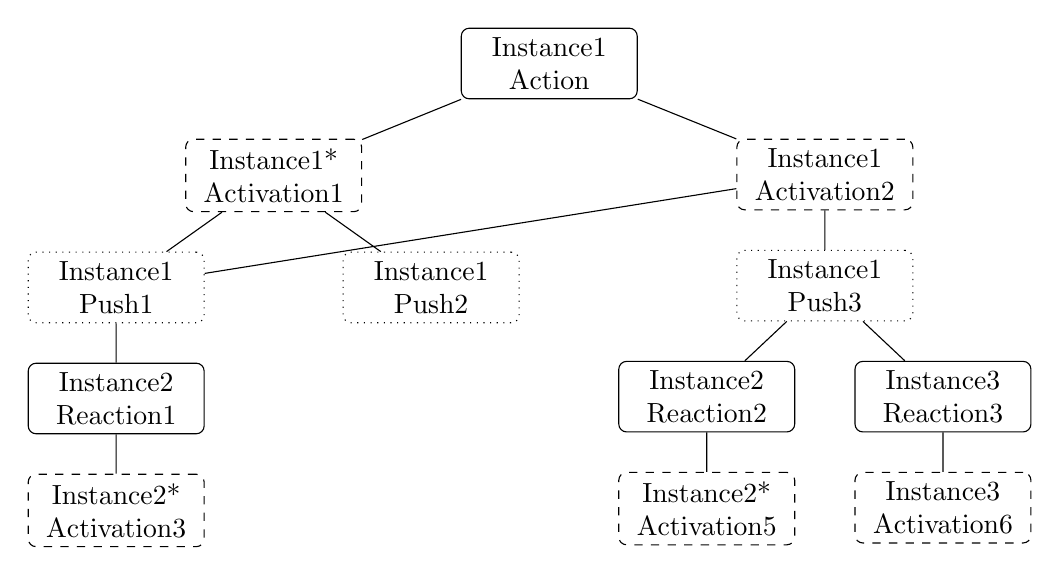
\begin{tikzpicture}[
    reaction/.style={rectangle, draw, rounded corners=1mm, text width=2cm,
        text centered, anchor=north},
    activation/.style={rectangle, draw, rounded corners=1mm, dashed, text width=2cm,
        text centered, anchor=north},
    push/.style={rectangle, draw, rounded corners=1mm, dotted, text width=2cm,
        text centered, anchor=north},
    level 1/.style={sibling distance=7.0cm},
    level 2/.style={sibling distance=4.0cm},
    level 3/.style={sibling distance=3.0cm},
    level distance=0.5cm, growth parent anchor=south
]
\node (Action) [reaction] {Instance1 Action}
  child {
    node (Activation01) [activation] {Instance1* Activation1}
    child {
      node (Push01) [push] {Instance1 Push1}
      child {
        node (Rection01) [reaction] {Instance2 Reaction1}
        child {
          node (Activation03) [activation] {Instance2* Activation3}
        }
      }
    }
    child {
      node (Push02) [push] {Instance1 Push2}
    }
  }
  child {
    node (Activation02) [activation] {Instance1 Activation2}
    child {
      node (Push03) [push] {Instance1 Push3}
      child {
        node (Rection02) [reaction] {Instance2 Reaction2}
        child {
          node (Activation04) [activation] {Instance2* Activation5}
        }
      }
      child {
        node (Rection03) [reaction] {Instance3 Reaction3}
        child {
          node (Activation05) [activation] {Instance3 Activation6}
        }
      }
    }
  }
;

\draw (Activation02) -- (Push01);

\end{tikzpicture}
%%}%
\caption{Example concrete action\label{concrete_action}}
\end{figure}

\begin{figure}
\centering
%%\resizebox{\textwidth}{!}{%
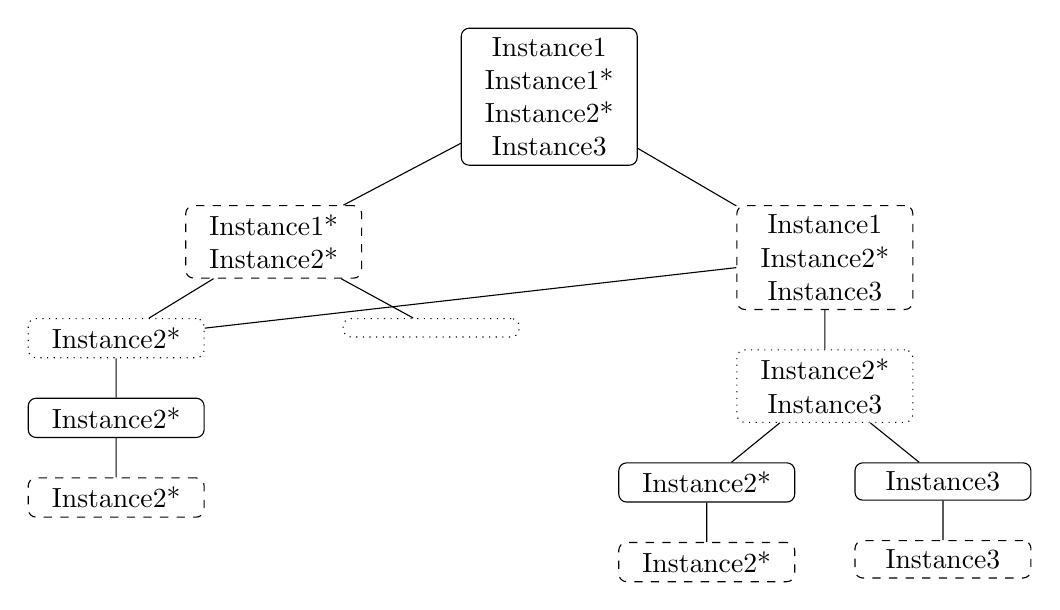
\begin{tikzpicture}[
    reaction/.style={rectangle, draw, rounded corners=1mm, text width=2cm,
        text centered, anchor=north},
    activation/.style={rectangle, draw, rounded corners=1mm, dashed, text width=2cm,
        text centered, anchor=north},
    push/.style={rectangle, draw, rounded corners=1mm, dotted, text width=2cm,
        text centered, anchor=north},
    level 1/.style={sibling distance=7.0cm},
    level 2/.style={sibling distance=4.0cm},
    level 3/.style={sibling distance=3.0cm},
    level distance=0.5cm, growth parent anchor=south
]
\node (Action) [reaction] {Instance1 Instance1* Instance2* Instance3}
  child {
    node (Activation01) [activation] {Instance1* Instance2*}
    child {
      node (Push01) [push] {Instance2*}
      child {
        node (Rection01) [reaction] {Instance2*}
        child {
          node (Activation03) [activation] {Instance2*}
        }
      }
    }
    child {
      node (Push02) [push] {}
    }
  }
  child {
    node (Activation02) [activation] {Instance1 Instance2* Instance3}
    child {
      node (Push03) [push] {Instance2* Instance3}
      child {
        node (Rection02) [reaction] {Instance2*}
        child {
          node (Activation04) [activation] {Instance2*}
        }
      }
      child {
        node (Rection03) [reaction] {Instance3}
        child {
          node (Activation05) [activation] {Instance3}
        }
      }
    }
  }
;

\draw (Activation02) -- (Push01);

\end{tikzpicture}
%%}%
\caption{Example instance set calculation\label{instance_sets}}
\end{figure}

The first step in analyzing a concrete action is to ensure that the directed graph is acyclic.
A cycle forms when a reaction activates itself through the set of concrete bindings or a getter calls itself.
In the example, the Instance1/Push1 is activated by both Activation1 and Activation2.

The second step in analyzing a concrete action is to determine which activations mutate the state of a component.
The current implementation uses a conservative static analysis of the body of an activate statement to determine if the activation mutates the state of the component.
These activations are marked with an asterisk (*) in figure~\ref{concrete_action}.

The third step is to compute a set of instances for each node in the concrete action.
If the node is not an activation, the set of instances is the union of the instances of its children.
If the node is an activation, the set of instances is the union of the instances of its children and the instance implied by the activation.
Figure~\ref{instance_sets} shows the instance set calculation for the concrete action in figure~\ref{concrete_action}.
The root shows that Instance1 does not change in at least one activation and may change in at least one activation, that Instance2 may change in every activation, and that Instance3 is ``read-only'' in this concrete action.

The fourth step is to check that a mutated instance appears in at most one child node instance set for the activation and push port nodes.
This check succeeds everywhere but Activation2 in figures~\ref{concrete_action}~and~\ref{instance_sets} as Instance2* appears in both children.
The activation and push port nodes represent activities that will be performed together.
That is, once control passes to an activation statement, all push ports and their bound reactions are activated.
In contrast, activations, as children of action and reaction nodes, represent mutually exclusive alternatives, i.e., at most one activation statement is executed per action/reaction body.
Thus, a mutated instance appearing in two or more children of an activation node or push port node indicates that the state of a component may be mutated in disparate ways leading to a non-deterministic state transition.

\section{Activations}

When executing a transaction, the run-time must execute the immutable phase of all implied state transitions before executing any of the mutable phases.
To accomplish this, the run-time uses a novel calling convention to create a list of deferred contexts and statements that represent the mutable phase of each state transition.
The immutable phase constructs the list and the mutable phase processes the list.
To present the calling convention, we first present some details about the run-time such as the ordinary calling convention and push ports.
We then describe the behavior of the calling convention and illustrate its behavior using a number of examples.

\paragraph{Ordinary calling convention.}
The ordinary call mechanism in the run-time is based on the C-decl calling convention.
It assumes the existence of an \emph{instruction pointer} which contains the address of the currently executing instruction and a \emph{base pointer} which points to a location in the stack which can be offset to access arguments and local variables.
A ordinary call in the language is accomplished through the following sequence:
\begin{enumerate}
\item (Caller) Push arguments onto the stack, left to right.
\item (Caller) Push the instruction pointer onto the stack and transfer control to the body of the function, method, action, reaction, getter, or initializer.
\item (Callee) Push the base pointer onto the stack and set the base pointer to the top of the stack.
\item (Callee) Reserve space on the stack for local variables.
\item (Callee) Execute the body of the function, method, etc.
\item (Callee) Pop the stack, pop and restore the base pointer, pop and restore the instruction pointer.
\item (Caller) Pop the arguments.
\end{enumerate}
The major difference between this calling convention and C-decl is that the arguments are pushed in the opposite order to match the semantics of Go.
The collection of arguments, previous instruction pointer, previous base pointer, and reserved space is called a \emph{stack frame} or a \emph{call frame}.
Figure~\ref{frame} shows the layout of a normal stack frame.
For this presentation, we assume that the stack grows down, i.e., the previous base pointer has a lower address in memory than the previous instruction pointer.

\begin{figure}
\centering
\resizebox{.5\textwidth}{!}{%
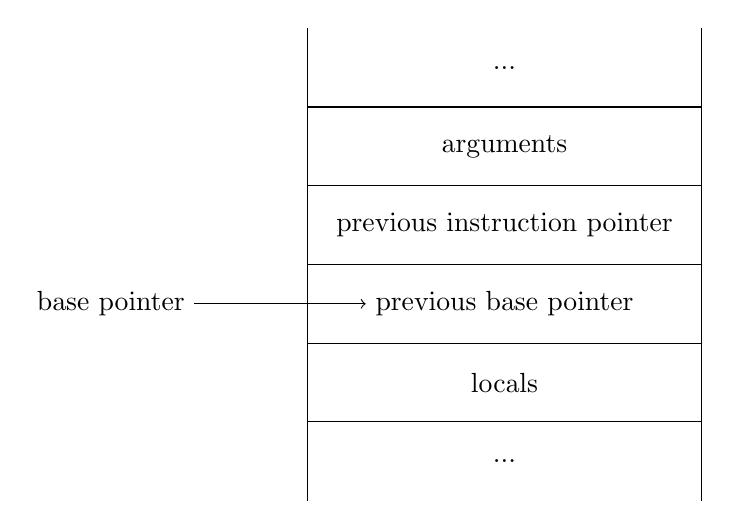
\begin{tikzpicture}
%% component boundary

\draw (0,1) -- (0,7);
\draw (5,1) -- (5,7);

\node at (2.5, 6.5) { ... };
\draw (0,6) -- (5,6);
\node at (2.5, 5.5) { arguments };
\draw (0,5) -- (5,5);
\node at (2.5, 4.5) { previous instruction pointer };
\draw (0,4) -- (5,4);
\node (pbp) at (2.5, 3.5) { previous base pointer };
\draw (0,3) -- (5,3);
\node at (2.5, 2.5) { locals };
\draw (0,2) -- (5,2);
\node at (2.5, 1.5) { ... };

\node (bp) at (-2.5, 3.5) { base pointer };
\draw[->] (bp) -- (pbp);

\end{tikzpicture}
}%
\caption{Diagram of a stack frame\label{frame}.  The stack is depicted as growing down.}
\end{figure}

\paragraph{Push ports.}
A push port is a field in a component.
Physically, a push port is a pointer to a linked list that contains the component pointer/reaction pairs that are bound to the push port.
The run-time populates each push port before execution begins.

\paragraph{Synchronized two-phase calling convention.}
To prepare for the mutable phase, the immutable phase must preserve the stack frame (context) of the action or reaction that executes an activation statement and must record which activation statement was executed so that the same activation can be resumed in the mutable phase.
To accomplish this, we devised the \emph{synchronized two-phase calling convention} which is used to execute activation statements during the immutable phase.

As previously stated, the execution of an activation statement is split into an immutable phase and a mutable phase.
Recall that activation statements may only appear in actions and reactions.
After executing the immutable phase of an activation statement in a reaction, control must be returned to the calling activation statement so that it may activate other push ports.
After executing the immutable phase of an activation statement in an action, control must be returned to the run-time to begin the mutable phase.
In the ordinary calling convention, the call frame for the reaction would be popped, control would be returned to the caller, and the arguments would be popped.
To preserve the call frame for use during the mutable phase, the activation statement returns control to the caller without popping the frame and the caller does not pop the arguments.
Thus, the complete frame for the reaction is preserved on the stack.

Each deferred call frame is added to a list to make it available in the mutable phase.
Let $head$ be a variable containing a pointer, initially nil, which will serve as the head of a linked list.
Before the activation statement returns from the immutable phase, it sets the previous base pointer in the call frame to the value of $head$ and updates head to be the current base pointer which inserts the call frame into the list.
The run-time can iterate over the elements of the list by following the previous base pointer to access all of the call frames that are needed for the mutable phase.
If the list is empty ($head$ is nil), then no activation statement was executed and the mutable phase may be skipped.

The final piece of information that must be recorded is the activation statement or rather the body of the activation statement so that it is accessible in the mutable phase.
Before returning from the immutable phase, the activation statement records the body of the activation statement in the previous instruction pointer slot of the call frame.
It is safe to use the previous instruction pointer because it is not used beyond the immediate return.
Furthermore, it is at a fixed location which allows it to be accessed in any deferred call frame.

The synchronized two-phase calling convention is used when executing an activation statement and proceeds as follows:
\begin{enumerate}
\item Save the previous base pointer of the current stack frame in $bp$.
\item Set the previous base pointer of the current stack frame to the value of $head$.
\item Set $head$ to the value of the base pointer.
\item Save the previous instruction pointer of the current stack frame in $ip$.
\item Set the previous instruction pointer of the current stack frame to the body of the activation statement.
\item For each push port in the port call list:
  \begin{enumerate}
  \item Push the arguments to the push port onto the stack.\label{step1}
  \item For each component pointer/reaction pair in the push port:
    \begin{enumerate}
    \item Push the component pointer onto the stack.
    \item Copy the arguments prepared in~\ref{step1} onto the stack.
    \item Call the reaction.
    \end{enumerate}
  \end{enumerate}
\item Set the base pointer to the value of $bp$ and return control to the value of $ip$.
\end{enumerate}

The synchronized two-phase calling convention evaluates the arguments to a push port once and passes a copy to each bound reaction.
One alternative is to evaluate the arguments for each bound reaction.
This means that the arguments may not be evaluated, i.e., the push port is not bound to any reactions, or may be evaluated multiple times.
If the arguments contain an expression with side-effects, then the behavior of the code becomes dependent on composition.
While this may be desirable in some cases, we opted for making a port call resemble ordinary function call as much as possible.
This sentiment also influenced our decision to pass a copy of the arguments to each reaction as opposed to reusing the same set of prepared arguments.
Since each reaction starts with a copy of the arguments, it is free to manipulate them as allowed by the semantics of Go.
Furthermore, the arguments are available in the mutable phase which obviates the need to make local copies of arguments.
This approach assumes that copying arguments does not generate significant overhead.

%% After an activation statement calls the last push port, it makes temporary copies of the instruction pointer and base pointer of the caller.
%% It may then safely overwrite the base pointer to insert itself into the list of mutable phase call frames and it may safely overwrite the instruction pointer with the body of the activation statement.

The major caveat when using the synchronized two-phase calling convention is that it must be assumed that the stack pointer changes when calling a push port.
To illustrate why this is an issue, consider the case when a caller wishes to preserve the contents of a register.
One strategy is to push the contents of the register onto the stack, perform the call, and then pop the value from the stack into the register.
After calling a push port, the caller may no longer assume that the previous value of the register is at the top of the stack.
The easy work-around is to allocate local variables, i.e., variables whose addresses are relative to the base pointer instead of the stack pointer, for saving temporary values that must persists across a push port call.
In the same way, the variables used to iterate over the list of component/reaction pairs in a push port should be allocated as local variables so that they may survive the calls to the reactions.

\paragraph{The mutable phase.}
The mutable phase consists of executing all of the deferred activation statements.
The algorithm for doing so is as follows:
\begin{enumerate}
\item If the value of $head$ is nil, stop.  Otherwise, set the base pointer to the value in $head$.
\item Transfer control to the instruction indicated by the previous instruction pointer\label{transfer}.  Execution continues until the body of the activation statement implicitly or explicitly returns.
\item If the previous base pointer is nil, stop.  Otherwise, set the base pointer to the previous base pointer and go to \ref{transfer}.
\end{enumerate}

The algorithm iterates over the list of deferred call frames accessible through $head$.
The last element in the list is indicated by a previous base pointer that is nil.
Transfer is controlled to the previous instruction pointer which contains the body of the activation statement.

\begin{figure}
\centering
\resizebox{.75\textwidth}{!}{%
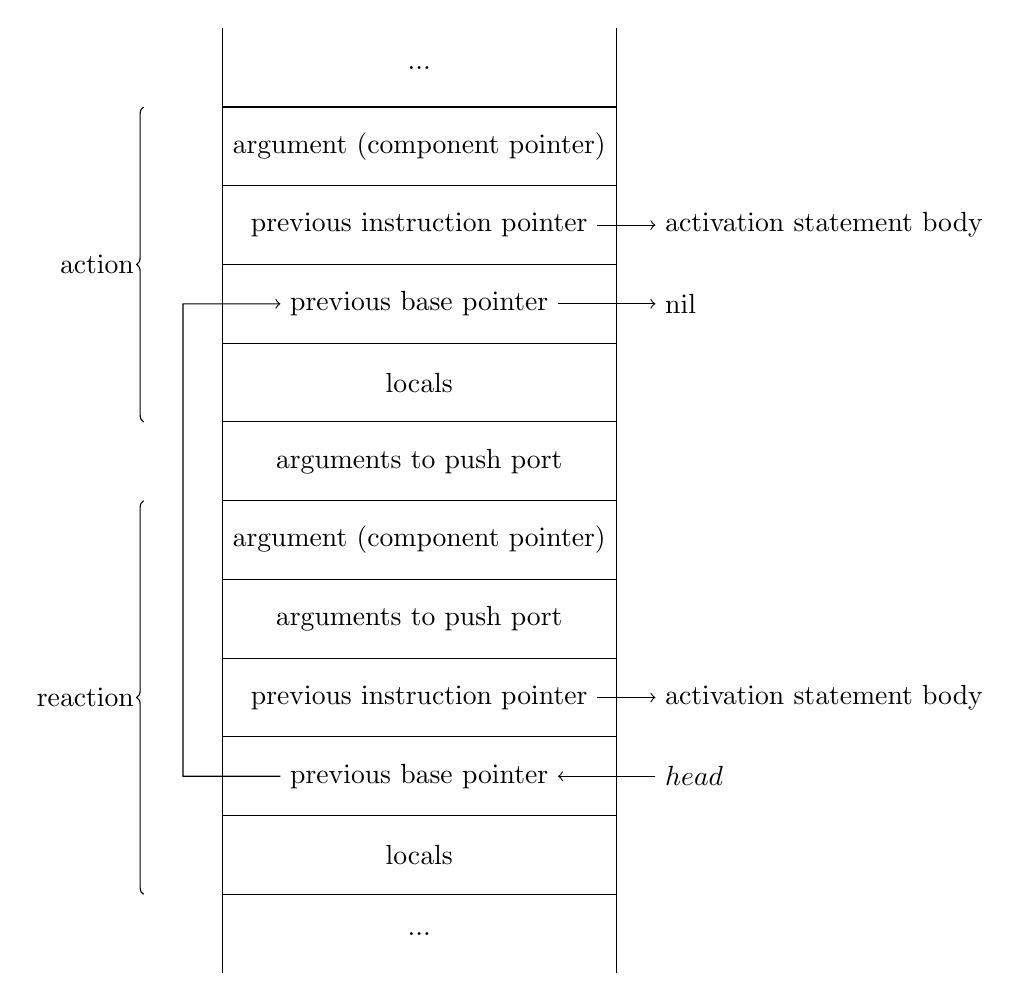
\begin{tikzpicture}
%% component boundary

\draw (0,-5) -- (0,7);
\draw (5,-5) -- (5,7);

\node at (2.5, 6.5) { ... };
\draw (0,6) -- (5,6);
\node at (2.5, 5.5) { argument (component pointer) };
\draw (0,5) -- (5,5);
\node (pip1) at (2.5, 4.5) { previous instruction pointer };
\draw (0,4) -- (5,4);
\node (pbp1) at (2.5, 3.5) { previous base pointer };
\draw (0,3) -- (5,3);
\node at (2.5, 2.5) { locals };
\draw (0,2) -- (5,2);
\node at (2.5, 1.5) { arguments to push port };
\draw (0,1) -- (5,1);
\node at (2.5, .5) { argument (component pointer) };
\draw (0,0) -- (5,0);
\node at (2.5, -.5) { arguments to push port };
\draw (0,-1) -- (5,-1);
\node (pip2) at (2.5, -1.5) { previous instruction pointer };
\draw (0,-2) -- (5,-2);
\node (pbp2) at (2.5, -2.5) { previous base pointer };
\draw (0,-3) -- (5,-3);
\node at (2.5, -3.5) { locals };
\draw (0,-4) -- (5,-4);
\node at (2.5, -4.5) { ... };

\node[anchor=west] (as1) at (5.5, 4.5) { activation statement body };
\draw[->] (pip1) -- (as1);
\node[anchor=west] (as2) at (5.5, -1.5) { activation statement body };
\draw[->] (pip2) -- (as2);

\draw[->] (pbp2) -- ++(-3,0) -- ++(0,6) -- (pbp1);

\node[anchor=west] (nil) at (5.5, 3.5) { nil };
\draw[->] (pbp1) -- (nil);

\node[anchor=west] (head) at (5.5, -2.5) { $head$ };
\draw[->] (head) -- (pbp2);

\draw[decorate,decoration={brace}] (-1,2) -- (-1,6) node[anchor=east,midway] { action };

\draw[decorate,decoration={brace}] (-1,-4) -- (-1,1) node[anchor=east,midway] { reaction };

\end{tikzpicture}
}%
\caption{Diagram of the stack after the immutable phase when an action activates a single reaction.\label{activation_ex_1}}
\end{figure}

\paragraph{Example:  one action, one reaction.}
Suppose an action activates a single push port that is bound to a single reaction and the reaction has a single activation that does not activate any push ports.
Figure~\ref{activation_ex_1} shows a diagram of the stack after the immutable phase for this scenario.
The stack contains two frames, one corresponding to the action and one corresponding to the reaction.
The $head$ variable points to the reaction frame which in turn points to the action frame using the previous base pointer slot.
The action frame points to nil indicating that it is the last frame in the list.
The previous instruction pointers point the bodies of the activation statements.
Between the frames are the push port arguments which duplicated for the call to the reaction.

\section{Heaps}

\section{Scheduler}








\section{Motivation}

An implementation of reactive components is necessary for at least three reasons.
First and foremost, an implementation tests the practicality of the model.
The act of implementing the model will reveal whether the assumptions upon which the model is founded can be realized using existing techniques.
Conversely, an implementation can suggest restrictions to the model that are necessary to produce an effective implementation.
An example of this was seen in chapter~\ref{model} where the component instance was used as proxy for its state variables for the purpose of determining which variables were involved in a transaction.
Implementation forces one to supply and consider details that can either qualify or disqualify a model as a practical engineering tool.
This is consistent with the emerging attitude in systems research that all new ideas and techniques must be accompanied by relevant tools and evaluations to show their feasibility.

Second, language support for a model is beneficial because it closes the semantic gap between reasoning and implementation.
The importance of language support can be seen in techniques like structured programming~\cite{dahl1972structured} and object-oriented programming~\cite{booch1982object}.
While these techniques can be applied in virtually any setting, their lasting utility is derived from their implementation in a variety of programming languages.
Providing language support for a model raises the level of abstraction and allows reasoning about a system directly from its specification instead of reasoning in one set of semantics while implementing in another which can be tedious and error-prone.
Language support allows developers to rely on the consistent application of the semantics of the model through strict enforcement, e.g., checking by a compiler.

Third, an implementation is necessary to demonstrate that the model can be applied successfully to real-world design and implementation problems.
That is, given a platform for reactive components, we can design, construct, and evaluate systems based on the reactive component paradigm.
Furthermore, we can evaluate critically the design and implementation processes that the model and platform encourage.
By comparing implementations of similar systems in two different models, we can gain insight into the strengths and weaknesses of the model.
These ideas will be explored further in section~\ref{evaluation}.

\section{Approach}
Our approach to implementing reactive components is to define a programming language for reactive components and implement that language in an interpreter.
The choice to implement an interpreter instead of a byte-code interpretation, i.e., a virtual machine, or a compiler was a matter of convenience as it avoids the code generation step.
However, this choice revealed something.
The programming language provides the syntax necessary to express all of the reactive component concepts:  state variables, actions, reactions, bindings, push ports, pull ports, and activation.

The development workflow, then, consists of three steps.
First, the developer defines a reactive system as a set of components in source files using a high-level language similar to the one used in the listings of section~\ref{model}.
Then the developer designates a top-level component that represents the system and compiles the source files to produce an $\alpha$-machine image.
Finally, the developer runs the system by loading an $\alpha$-machine with the image created in the previous step.

This approach has two desirable characteristics.
First, the virtual machine facilitates a separation of concerns between syntax and operational semantics.
The issues of compilation and execution can be divided by the interface provided by the virtual machine.
Thus, we can focus on implementing an $\alpha$-machine without considering the high-level language used to encode component definitions.
Similarly, we can focus on the translation of a high-level language for component definitions to the language of the virtual machine without considering the details of how the virtual machine is implemented.
Second, writing a compiler for a virtual machine is often easier than writing a compiler for a physical machine.
The target provided by a virtual machine is often at a higher-level of abstraction than a physical machine and can contain features and instructions that simplify or optimize certain tasks.
%% For example, the Java virtual machine contains an instruction for creating new objects.
A design based on a virtual machine will allow us to focus on the semantics of reactive programs instead of the complexities of processor architecture.

\paragraph{Static system assumption.}
To make implementation tractable, we will assume that the systems to be implemented have a static topology meaning that all reactive components are statically allocated.
Both finite state and infinite state (subject to system resource limits) reactive components are permitted, but both the number and configurations of reactive components in a system are fixed.
This is equivalent to systems that assume a fixed number of actors and is roughly equivalent to systems that assume a fixed number of threads.
These assumptions are common in embedded and real-time systems due the combination of limited resources and a need for predictability.
We also believe these assumptions are common in less constrained environments as the number of threads is often fixed by the design, e.g., only a fixed number of concurrent activities is needed, or the number of threads is limited by the number of available physical cores.
Thus, even with the static system assumption, an implementation of the model is still applicable to many systems of interest.
We leave implementation of extensions that facilitate the dynamic creation and binding of reactive components for future work.

\section{Programming Language}
Describe the reactive/transformational split and dismiss the transformational.
Assignment.
Describe how actions, reactions, etc. appear in the language.
Enforcing the immutable/mutable phase split.

\section{Semantic Checking}
Describe the algorithms used to enforce the semantics of reactive components.
\begin{enumerate}
\item Enumerate instances
\item Enumerate bindings
\item Enumerate concrete actions
\item Check for non-determinism
\item Check that all pull ports are satisfied
\end{enumerate}

\section{Runtime}
Activations
Scheduler
Garbage collector should be deferred to advance features



\section{BEGINNING OF UNADOPTED MATERIAL FROM PROPOSAL}

\paragraph{Compilation.}
To facilitate a design and development process based on composition and decomposition, we require a high-level language that resembles the model and examples presented in section~\ref{model}.
The goal of the compiler, then, is to translate the high-level language to the language of the $\alpha$-machine.
%% Complication typically consists of five phases corresponding to scanning, parsing, semantic analysis, optimization, and code generation.
In addition to conventional semantic analysis, e.g., type checking, the compiler will check that the reactive system is well-defined and provide a concurrency analysis to be used during scheduling.
%% Optimization is beyond the scope of this research.

Substitutional equivalence provides the logical foundation for testing well-definedness.
A system is represented as a top-level reactive component.
The input and output ports original to the top-level component can be converted to internal ports since the top-level component does not need an external interface.
Substitutional equivalence allows the declarations of member components to be replaced with their definitions according to the procedure outlined in section~\ref{model}.
This process can be repeated until all member components are ``inlined'' resulting in a top-level component that only contains state variables, internal ports, $\alpha$-statements, $\beta$-statements, and $\gamma$-statements.
At this point, all internal ports, $\gamma$-statements, and $\beta$-statements can be eliminated by substituting definitions.
The resulting top-level component only contains state variables and $\alpha$-statements.
To be a faithful implementation of the model, each $\alpha$-statement must be a deterministic state transformation.
The main challenge, then, lies in the co-design of a transformational language and checks for deterministic assignment.

At a high level, we desire to treat the transformation specified by an $\alpha$-statement as a function that maps a value representing the current state to a value representing the next state because it leads to a simple decidable check.
An $\alpha$-statement then consists of five parts:  a precondition list, a precondition function, an assignment list, an argument list, and an effect function.
The precondition list and argument list are lists of readable objects that form the arguments of the precondition function and effect function, respectively.
The assignment list is a list of writable objects that are assigned the values produced by the effect function (state variables that are not named in the assignment list retain their previous values and ports that are not named in the assignment list are undefined).
There is no notion of state or assignment inside the effect function, which thus resembles a pure functional or applicative program.
A conservative but decidable check, then, is to ensure that a writable object appears at most once in the assignment list.

%%Another concept implicit in the semantics of functional languages and their data structures is freedom from aliasing.
The approach outlined above hinges on the semantics of writable objects.
We define a writable object to be the name for an implied set of storage locations.
All elements in the set of storage locations for a scalar variable are updated in an assignment to the variable.
In contrast, only a subset of the set of storage locations for aggregate variables such as arrays and records may be updated in an assignment.
Variables can also name linked data structures where the set of locations is the transitive closure of a points-to analysis~\cite{hind2001pointer}.

For well-definedness, we require that the implied sets of storage locations for all writable objects be disjoint.
Thus, an assignment to two different variables in an $\alpha$-statement cannot update the same memory location.
The challenge then is to show that this condition holds initially and that it holds after the execution of each $\alpha$-statement.
This is the subject of pointer analysis~\cite{hind2001pointer} which is undecidable in general.
Components that communicate by passing data by reference as opposed to by value obviously violate this condition since multiple components may then reference the same memory locations.
Thus, data passed by reference through ports must have semantics that prevent concurrent updates, e.g., constant (read-only), copy-on-write, etc.
The goal then is to place appropriate restrictions on the language so as to make pointer analysis feasible and enable the safe sharing of data across ports.

To achieve the general approach outlined above, an approach to persistent data structures~\cite{driscoll1989making} and copy elimination~\cite{gopinath1989copy} is needed.
A persistent data structure is one in which updates and queries can be made to any version, e.g., lists in LISP, Scheme, Haskell, etc.
Persistent data structures match the semantics of existing functional programming languages since they allow variables to be treated as immutable values.
In contrast, an ephemeral data structure is one in which updates and queries can only be to the most recent version.
Ephemeral data structures are common in imperative languages and typically have simpler designs~\cite{okasaki1999purely}.
Copy elimination attempts to replace copying with in-place modification when it can be shown that the old value of a variable is no longer needed.
Copy elimination is often used for large aggregate data structures, e.g., arrays, that resist efficient persistent implementations.

An approach that to our knowledge has not been attempted is to restrict a functional language solely to ephemeral data structures.
We define an \emph{ephemeral function} to be a function with an implementation (i.e., \emph{schedule of operations}) that allows all data structures to be treated as ephemeral.
This approach has the potential to be more efficient since variables may be updated without copying.
Functions with no ephemeral schedule must explicitly introduce copying, which is beneficial since it makes the developer aware of such potentially costly operations.
Ephemeral functions may \emph{compose}, meaning that ephemerality may be established solely from the definition of a function and the signatures of any called functions.
The challenge then is to develop an analysis to determine if a function is ephemeral and design the language of $\alpha$-statement transformations based on this analysis.

The goal of concurrency analysis is to determine which $\alpha$-statements are independent and therefore can be executed concurrently.
Using the formulation above, we associate with each $\alpha$-statement a set of objects given by forming the union of the precondition list, assignment list, and argument list (called the $\alpha$-statement's \emph{implied objects}).
Two $\alpha$-statements are independent if their sets of implied objects are disjoint.

%% One idea is to treat $\alpha$-statements as ``pure'' data-flow programs which have properties that are conducive to analysis.
%% The structure present when compiling can also provide insights into the pointer analysis problem.
%% For example, one could envision a heap-per-component strategy where each heap is considered as an extra variable.
%% Passing a pointer through a port involves transferring the ownership of an object from one heap to another heap or set of heaps.
%% Thus, the language might include two pointer types corresponding to the pointers ability to be passed to another component.
%% This idea might be extended resulting in multiple heaps per component.

%% To be a faithful implementation of the model, each $\alpha$-statement must be a deterministic state transformation.
%% Thus, a compiler or verifier of $\alpha$-machine bytecode must be able to prove this property and the language of $\alpha$-statements must be designed around this constraint.
%% A conservative but straightforward approach to proving determinism for variables in static storage is to check that a state variable is written at most once in all possible executions of an $\alpha$-statement.
%% Existing techniques, e.g., control flow analysis, are adequate for this purpose.
%% Proving determinism for variables allocated on the heap requires pointer analysis, e.g., shape analysis~\cite{larus1988detecting}, an area of ongoing research.
%% Most likely, the language of $\alpha$-statements will need to be restricted to make pointer analysis feasible.

%% A compiler for this language takes as input reactive components constituting the system and uses the aforementioned techniques based on substitutional equivalence and simplification to produce an $\alpha$-machine program.
%% In addition to the aforementioned determinism check, the compiler should check for appropriate port usage, e.g., input ports are read while output ports are written, and port consistency (static versus dynamic).
%% The additional structure present when compiling from a high-level language will be useful when reporting errors related to non-deterministic assignment statements, perhaps by indicating the error using the same information presented in the block diagram of figure~\ref{clocksys_component_graphic} or the $\alpha$-forest diagram of \ref{clocksys_component_alpha}.
%% The compiler can also help in design as it can perform concurrency analysis which the developer might use to identify bottlenecks and reactive components or systems that are good candidates for redesign.


%% The $\alpha$-machine processes a low-level language similar to Java bytecode.
%% The reactive program given to an $\alpha$-machine lacks the structural elements, i.e., components, ports, $\beta$-statements, and $\gamma$-statements, needed to facilitate a design and development process based on composition and decomposition.

%% We believe that the gross structure for reactive components presented in the examples of section~\ref{model} is adequate for structuring systems.
%% The main challenge lies in the design of a transformational language that will facilitate the determinism checks.
%% One idea is to treat $\alpha$-statements as ``pure'' data-flow programs which have properties that are conducive to analysis.
%% The structure present when compiling can also provide insights into the pointer analysis problem.
%% For example, one could envision a heap-per-component strategy where each heap is considered as an extra variable.
%% Passing a pointer through a port involves transferring the ownership of an object from one heap to another heap or set of heaps.
%% Thus, the language might include two pointer types corresponding to the pointers ability to be passed to another component.
%% This idea might be extended resulting in multiple heaps per component.

%% A system is represented as a top-level reactive component.
%% Substitutional equivalence allows the declarations of member components to be replaced with their definitions according to the procedure outlined in section~\ref{formalization}.
%% This process can be repeated until all member components are ``inlined'' resulting in a top-level component that only contains state variables.
%% The input and output ports original to the top-level component can be converted to internal ports since the top-level component does not need an external interface.
%% At this point, all internal ports, $\gamma$-statements, and $\beta$-statements can be eliminated by substituting definitions.
%% The resulting top-level component only contains state variables and $\alpha$-statements.

%% \begin{figure}
%% {
%% \input workflow.tex
%% \centerline{\box\graph}
%% }
%% \caption{A compilation workflow for reactive components\label{workflow}}
%% \end{figure}

%% Figure~\ref{workflow} shows our proposed compilation workflow for reactive components.
%% The goal of the workflow is to transla

%% The workflow begins with the definition of the components and the designation (*) of one component as the top-level component that will represent the system.
%% Substitutional equivalence allows the declarations of member components to be replaced with their definitions according to the procedure outlined in section~\ref{formalization}.
%% This process can be repeated until all member components are ``inlined'' resulting in a top-level component that only contains state variables.
%% The input and output ports original to the top-level component can be converted to internal ports since the top-level component does not need an external interface.
%% At this point, all internal ports, $\gamma$-statements, and $\beta$-statements can be eliminated by substituting definitions.
%% The resulting top-level component only contains state variables and $\alpha$-statements.

%% The top-level component is then subjected to semantic analysis to determine if the system is well-defined.

%% The final step of compilation generates an $\alpha$-machine image which contains static allocated variables, executable code for realizing the $\alpha$-statements, and schedule analysis indicating which $\alpha$-statements can be executed concurrently.
%% The $\alpha$-machine image can then be instantiated to produce an executing instance of the reactive system.

\paragraph{$\alpha$-machine.}
We propose a virtual machine, called an $\alpha$-machine, capable of executing systems expressed as a single top-level component containing only state variables and $\alpha$-statements.
An $\alpha$-machine has five parts:
\begin{enumerate}
\item The \emph{data section} contains all of the statically allocated state variables.
\item The \emph{heap} contains dynamically allocated state variables.
\item The \emph{program} contains the code necessary to implement the $\alpha$-statements.
\item The \emph{stack} contains dynamic storage for function calls and expression evaluation.
\item The \emph{scheduler} selects and executes $\alpha$-statements.
\end{enumerate}
For simplicity, we will limit the design to a stack-based machine since code generation for stack-based machines is straightforward.
Our approach to dynamic allocation, garbage collection, etc. will be shaped by the transformational language used to encode $\alpha$-statements.


%% \paragraph{Program.}
%% To be a faithful implementation of the model, each $\alpha$-statement must be a deterministic state transformation.
%% Thus, a compiler or verifier of $\alpha$-machine bytecode must be able to prove this property and the language of $\alpha$-statements must be designed around this constraint.
%% A conservative but straightforward approach to proving determinism for variables in the data section is to check that a state variable is written at most once in all possible executions of an $\alpha$-statement.
%% Existing techniques, e.g., control flow analysis, are adequate for this purpose.
%% Proving determinism for variables allocated on the heap requires pointer analysis, e.g., shape analysis~\cite{larus1988detecting}, an area of ongoing research.
%% Most likely, the language of $\alpha$-statements will need to be restricted to make pointer analysis feasible.

%% \paragraph{Scheduler.}
Of primary interest to this research is the scheduler.
The scheduler selects $\alpha$-statements and executes them based on their preconditions.
Furthermore, the scheduler must be fair meaning that it cannot indefinitely postpone the selection of an $\alpha$-statement.
One way of measuring the efficiency of a scheduler is to compare the number of preconditions that evaluate to true to the total number of evaluated preconditions.
Similarly, one could measure the time spent evaluating and reevaluating preconditions to the time spent evaluating effects.
Schedulers can also be compared using other criteria such as responsiveness, fairness, cache-awareness, context-switches, etc.
%% Using the pointer analysis techniques outlined above, one can also analyze the relationships between $\alpha$-statements to determine which $\alpha$-statements are independent meaning that they operate on disjoint sets of state variables (read and write).
Independent $\alpha$-statements can be executed concurrently prompting the development of a concurrent $\alpha$-machine and concurrent schedulers.
A concurrent scheduler should take advantage of the static structure latent in reactive components and the dynamic behavior of the system being executed when making scheduling decisions.

%% \paragraph{Compilation.}
%% The $\alpha$-machine processes a low-level language similar to Java bytecode or assembly language.
%% The reactive program given to an $\alpha$-machine lacks the structural elements, i.e., components, ports, $\beta$-statements, and $\gamma$-statements, needed to facilitate a design and development process based on composition and decomposition.
%% Thus, to make developing reactive programs easier, we also require a high-level language that more closely resembles the model and examples presented in section~\ref{model}.
%% A compiler for this language takes as input reactive components constituting the system and uses the aforementioned techniques based on substitutional equivalence and simplification to produce an $\alpha$-machine program.
%% In addition to the aforementioned determinism check, the compiler should check for appropriate port usage, e.g., input ports are read while output ports are written, and port consistency (static versus dynamic).
%% The additional structure present when compiling from a high-level language will be useful when reporting errors related to non-deterministic assignment statements, perhaps by indicating the error using the same information presented in the block diagram of figure~\ref{clocksys_component_graphic} or the $\alpha$-forest diagram of \ref{clocksys_component_alpha}.
%% The compiler can also help in design as it can perform concurrency analysis which the developer might use to identify bottlenecks and reactive components or systems that are good candidates for redesign.

%% We believe that the gross structure for reactive components presented in the examples of section~\ref{model} is adequate for structuring systems.
%% The main challenge lies in the design of a transformational language that will facilitate the determinism checks.
%% One idea is to treat $\alpha$-statements as ``pure'' data-flow programs which have properties that are conducive to analysis.
%% The structure present when compiling can also provide insights into the pointer analysis problem.
%% For example, one could envision a heap-per-component strategy where each heap is considered as an extra variable.
%% Passing a pointer through a port involves transferring the ownership of an object from one heap to another heap or set of heaps.
%% Thus, the language might include two pointer types corresponding to the pointers ability to be passed to another component.
%% This idea might be extended resulting in multiple heaps per component.

\paragraph{Summary.}
In this section, we have proposed to implement the model described in section~\ref{model} for systems with static topologies.
We proposed to develop a virtual machine called an $\alpha$-machine that executes a reactive component consisting solely of state variables and $\alpha$-statements.
The $\alpha$-machine will be a concurrent $\alpha$-machine.
We also proposed to develop a high-level language for specifying reactive components and a compiler that translates the specifications into an $\alpha$-machine program.
The main challenge is the design of the high-level language, which must be subject to an analysis for deterministic assignment.

%% POSIX environment, possibly bare metal
